\documentclass[tikz, border=15pt]{standalone}
\usepackage{amsmath}
\usepackage{amssymb}
\usetikzlibrary{calc, angles, quotes, arrows.meta}
\usetikzlibrary{decorations.pathreplacing, angles, quotes}

% Define custom colors
\definecolor{axisgreen}{RGB}{46, 139, 87}
\definecolor{axisblue}{RGB}{0, 0, 255}
\definecolor{lightzaxis}{RGB}{180, 200, 255}
\definecolor{frustumgray}{RGB}{240, 240, 240}

\begin{document}

% ==========================================
% IMAGE 1: y-z plane cross-section
% ==========================================
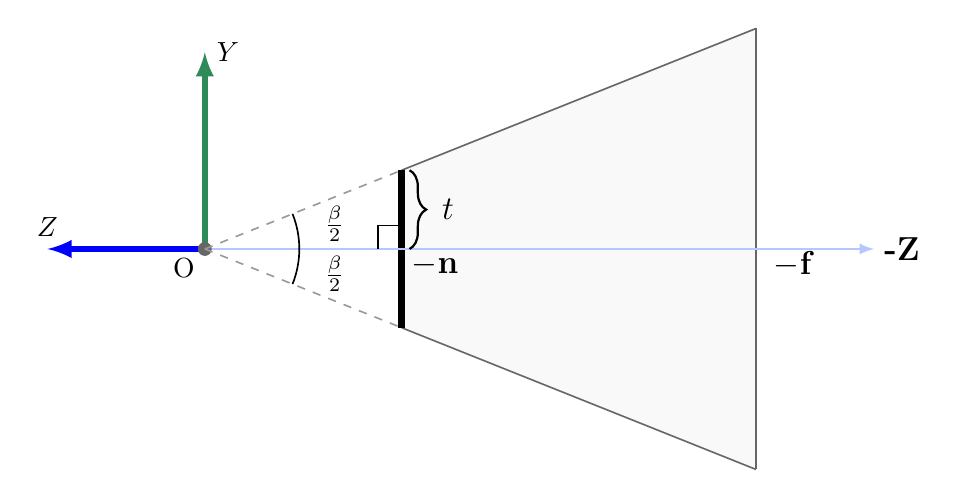
\begin{tikzpicture}[>=latex, font=\normalsize, line width=0.6pt]
    % Dimensions
    \def\L{7}    % Length to the far plane
    \def\n{2.5}  % Length to the near plane
    \def\H{2.8}  % Half-height of the frustum at the far plane
    \def\h{1}    % Half-height at the near plane (\H * \n / \L)

    % 1. Frustum shape (shaded area)
    \fill[frustumgray, opacity=0.4] (\n, \h) -- (\L, \H) -- (\L, -\H) -- (\n, -\h) -- cycle;

    % 2. Frustum outlines
    \draw[black!60] (\n, \h) -- (\L, \H);
    \draw[black!60] (\n, -\h) -- (\L, -\H);
    \draw[black!60] (\L, -\H) -- (\L, \H);

    % Near plane (thick line)
    \draw[line width=2.5pt] (\n, -\h) -- (\n, \h);

    % Depth labels for near and far planes
    \node[right, font=\large\bfseries] at (\n, -0.2) {$\mathbf{-n}$};
    \node[right, font=\large\bfseries] at (\L + 0.1, -0.2) {$\mathbf{-f}$};

    % Center -Z axis line extending through the frustum
    \draw[lightzaxis, -latex, line width=0.8pt] (0,0) -- (\L+1.5, 0) node[right, text=black, font=\large\bfseries] {-Z};

    % 3. Axes (Colored)
    \draw[axisblue, -latex, line width=2pt] (0,0) -- (-2,0) node[above, text=black] {$Z$};
    \draw[axisgreen, -latex, line width=2pt] (0,0) -- (0,2.5) node[right, text=black] {$Y$};
    \fill[black!60] (0,0) circle (2.5pt) node[below left, text=black] {O};

    % 4. Coordinates
    \coordinate (O) at (0,0);
    \coordinate (T) at (\L, \H);   % Top right
    \coordinate (B) at (\L, -\H);  % Bottom right
    \coordinate (M) at (\L, 0);    % Middle right
    \coordinate (NT) at (\n, \h);  % Near top
    \coordinate (NB) at (\n, -\h); % Near bottom

    % 5. Dashed projection lines to origin
    \draw[dashed, black!40] (O) -- (NT);
    \draw[dashed, black!40] (O) -- (NB);

    % 1. Origin to near plane (distance n)
    \draw[decorate, decoration={brace, amplitude=6pt, mirror}, thick] 
        (\n + 0.1, 0) -- (\n+ 0.1, \h) node[midway, right=8pt, font=\large] {$t$};
    

    % 7. Right Angle Marker
    \draw (\n-0.3, 0) -- (\n-0.3, 0.3) -- (\n, 0.3);

    % 8. Angles
    \pic[draw, "$\frac{\beta}{2}$", angle eccentricity=1.4, angle radius=1.2cm] {angle = M--O--T};
    \pic[draw, "$\frac{\beta}{2}$", angle eccentricity=1.4, angle radius=1.2cm] {angle = B--O--M};
    
\end{tikzpicture}

\end{document}